\section{Parcours différenciés}
\textbf{\color{red}Question : Doit-on laisser les noms et prénoms des élèves?}
\subsection{Parcours différenciés autour de la symétrie centrale}
\subsubsection*{Fiche d'exercice}\label{parcours_symetrie_centrale}
\begin{figure}[!h]
	\center{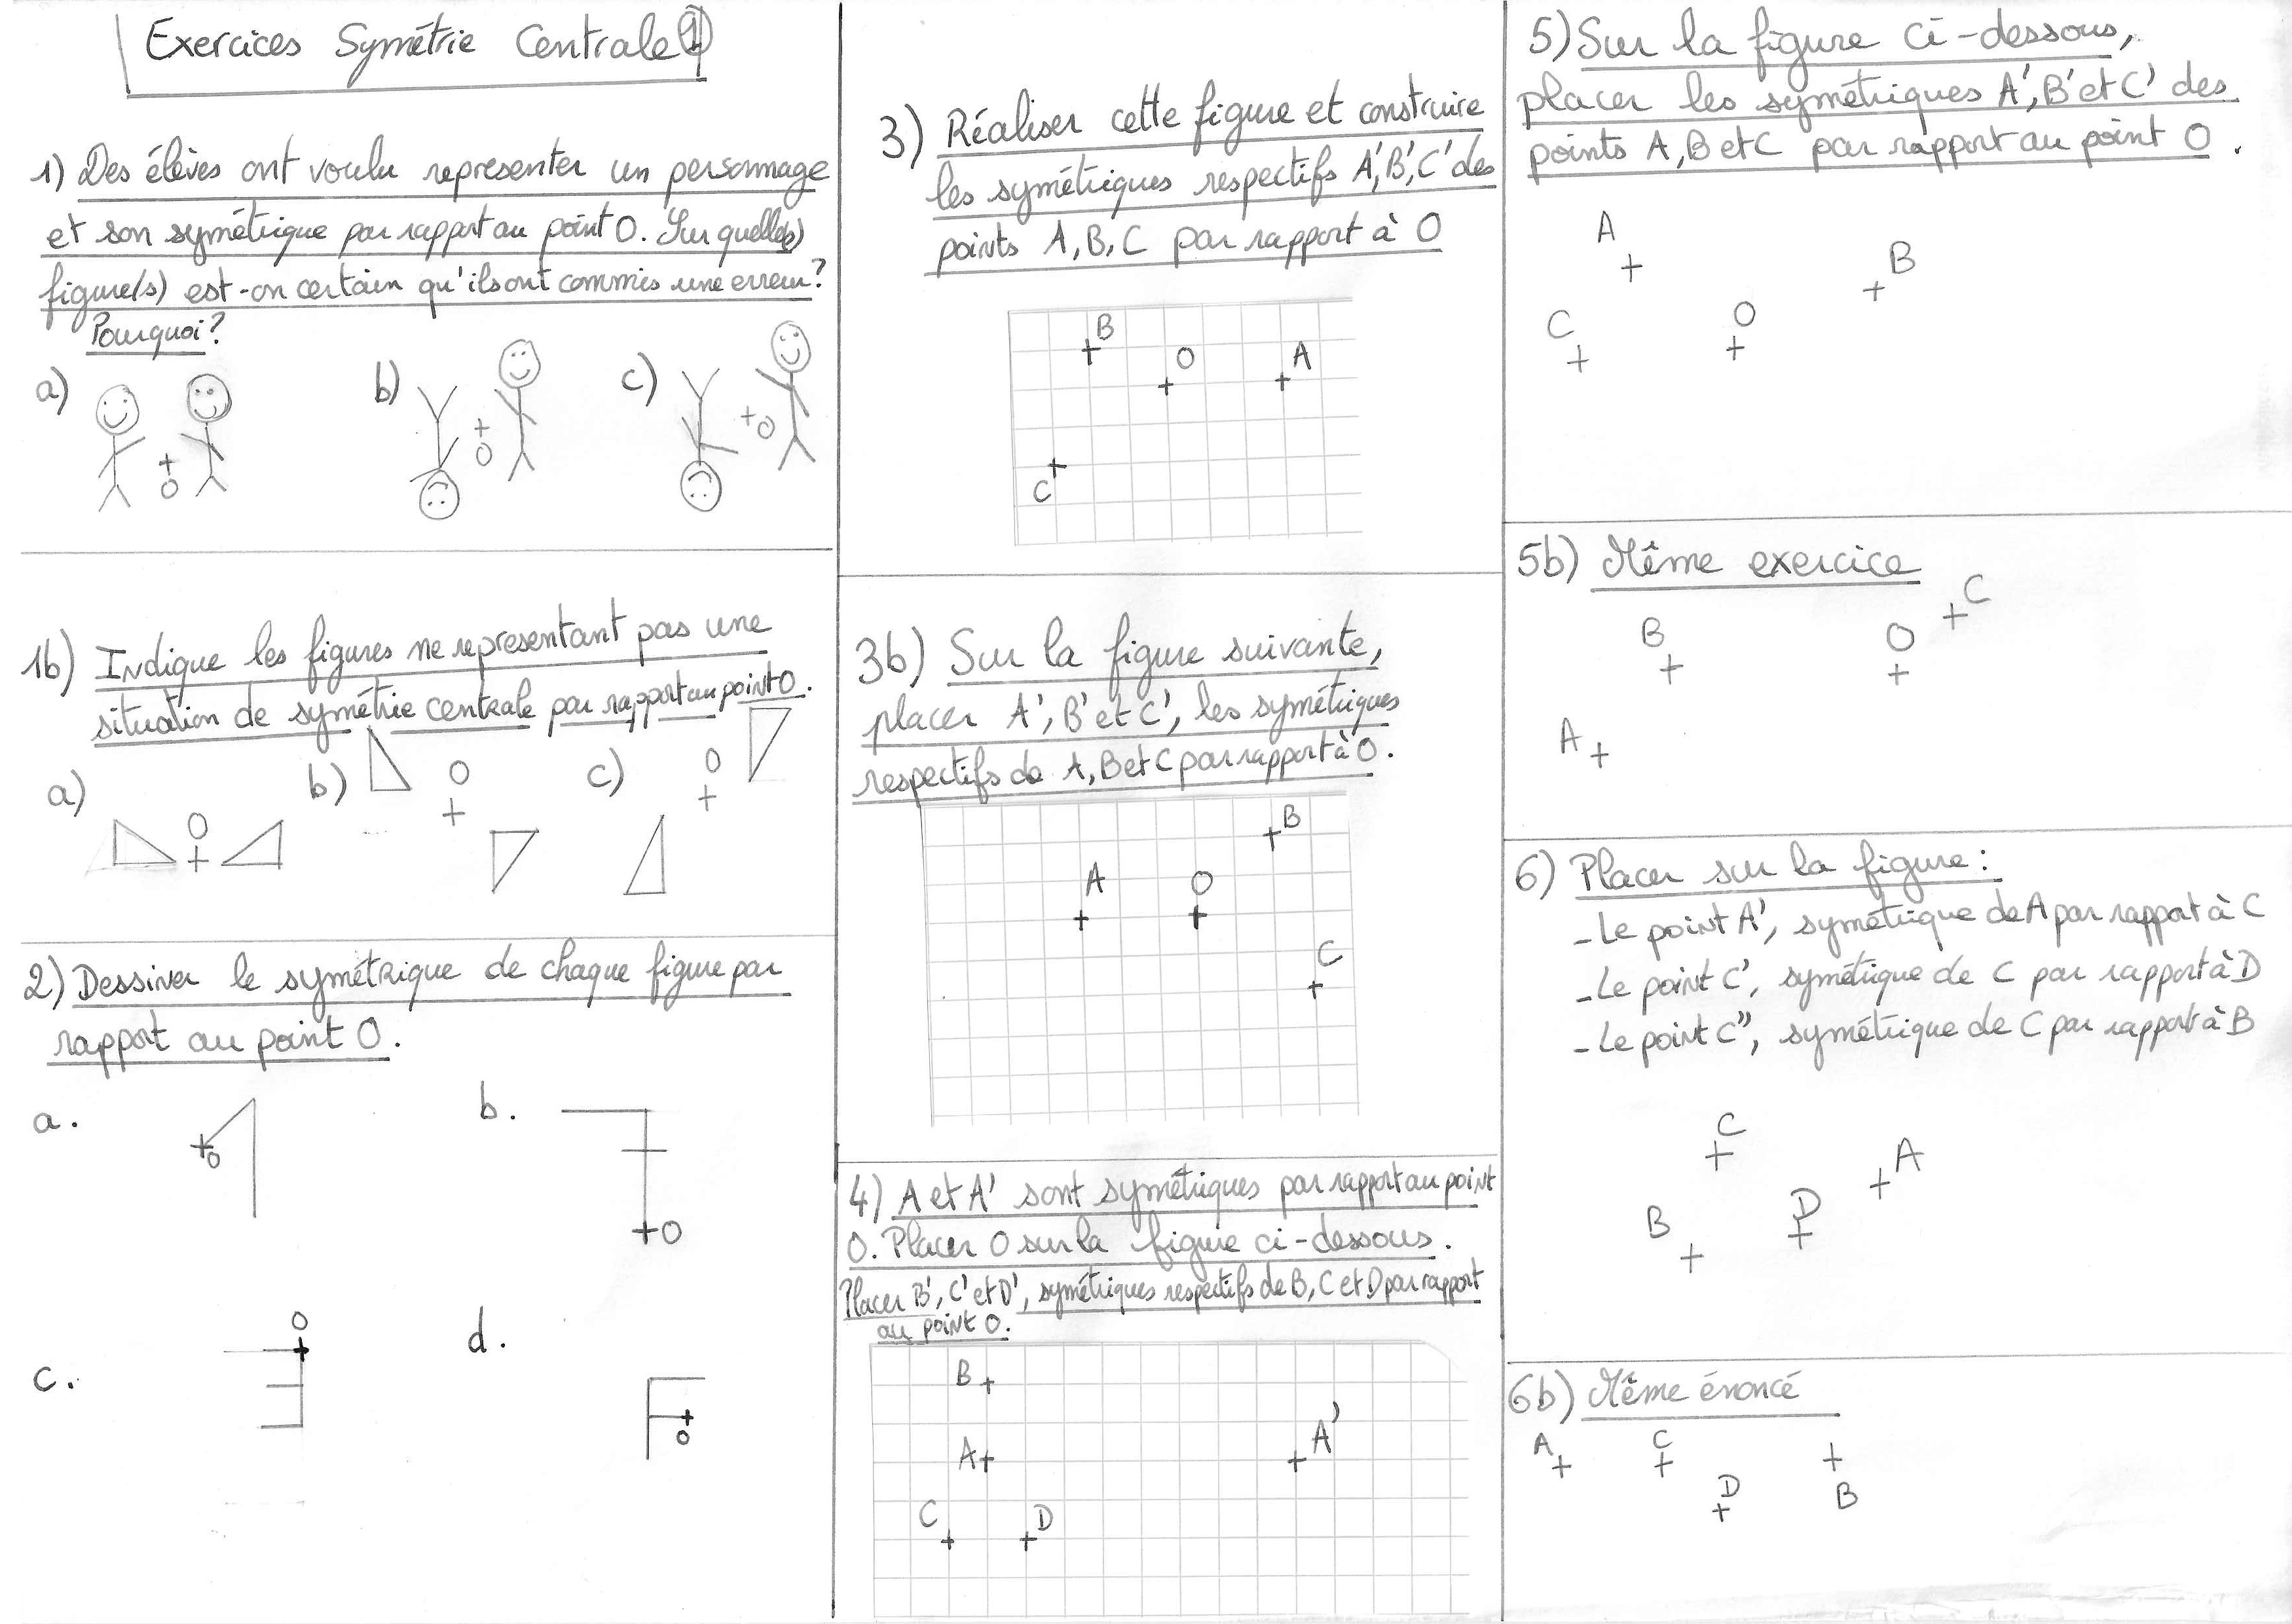
\includegraphics[scale=0.5]{img/Parcours_symetrie_julia1.jpg}}
\end{figure}
\subsubsection*{Parcours}
\subsubsection*{Productions d'élèves}\label{Prod_eleves_ju}
\paragraph{Parcours différencié : copies d'élèves de 5\up{ème} \\}
\textbf{\color{red}Note : Productions à scanner}
Layana est une élève qui manque de confiance en elle et qui a tendance  baisser les bras et à se dissiper si elle ne comprend pas immédiatement les clefs de l'exercice. Sur les travaux en autonomie via des parcours différenciés, j'ai remarqué qu'elle prenait plus de temps avant de demander de l'aide à ses camarades ou à moi. Elle a également modifié son attitude face aux difficultés en ciblant ses questions alors qu'elle adoptait l'attitude "Je ne comprends rien" auparavant.\\
Ilyes est un élève en grande difficulté au premier trimestre, avec un comportement perturbateur (prise de parole, bavardages, pas de travail). Son comportement s'est fortement amélioré au second trimestre. Il fait partie du dispositif \textit{Fiche de suivi}, ce qui a probablement eu un impact important sur son travail. Mes collègues m'indiquent cependant qu'ils ne remarquent pas des progrès aussi importants dans leurs matières, notamment sur la capacité à travailler en autonomie.\\
Dahlia est une élève à fort caractère qui a besoin d'attention face aux difficultés. Il s'agit cependant d'une élève plus à l'aise en mathématiques que la plupart de ses camarades. Suite à l'instauration des parcours différenciés, elle a gagné en autonomie mais continue de se braquer si elle n'obtient pas une aide du professeur. En revanche, elle a adopté le rôle de tuteur pour deux élèves en difficultés et a améliorer son expression orale. Il s'agit d'une des élèves qui m'ont convaincue de mettre en place d'autres supports de différenciation, notamment pour débloquer les élèves.
\paragraph{Evaluation sommative symétrie centrale : copies d'élèves de 5\up{ème}\\}
\textbf{\color{red}Note : Productions à trier et à commenter}
%\begin{figure}[h]
%	\centering
%	\subfloat{{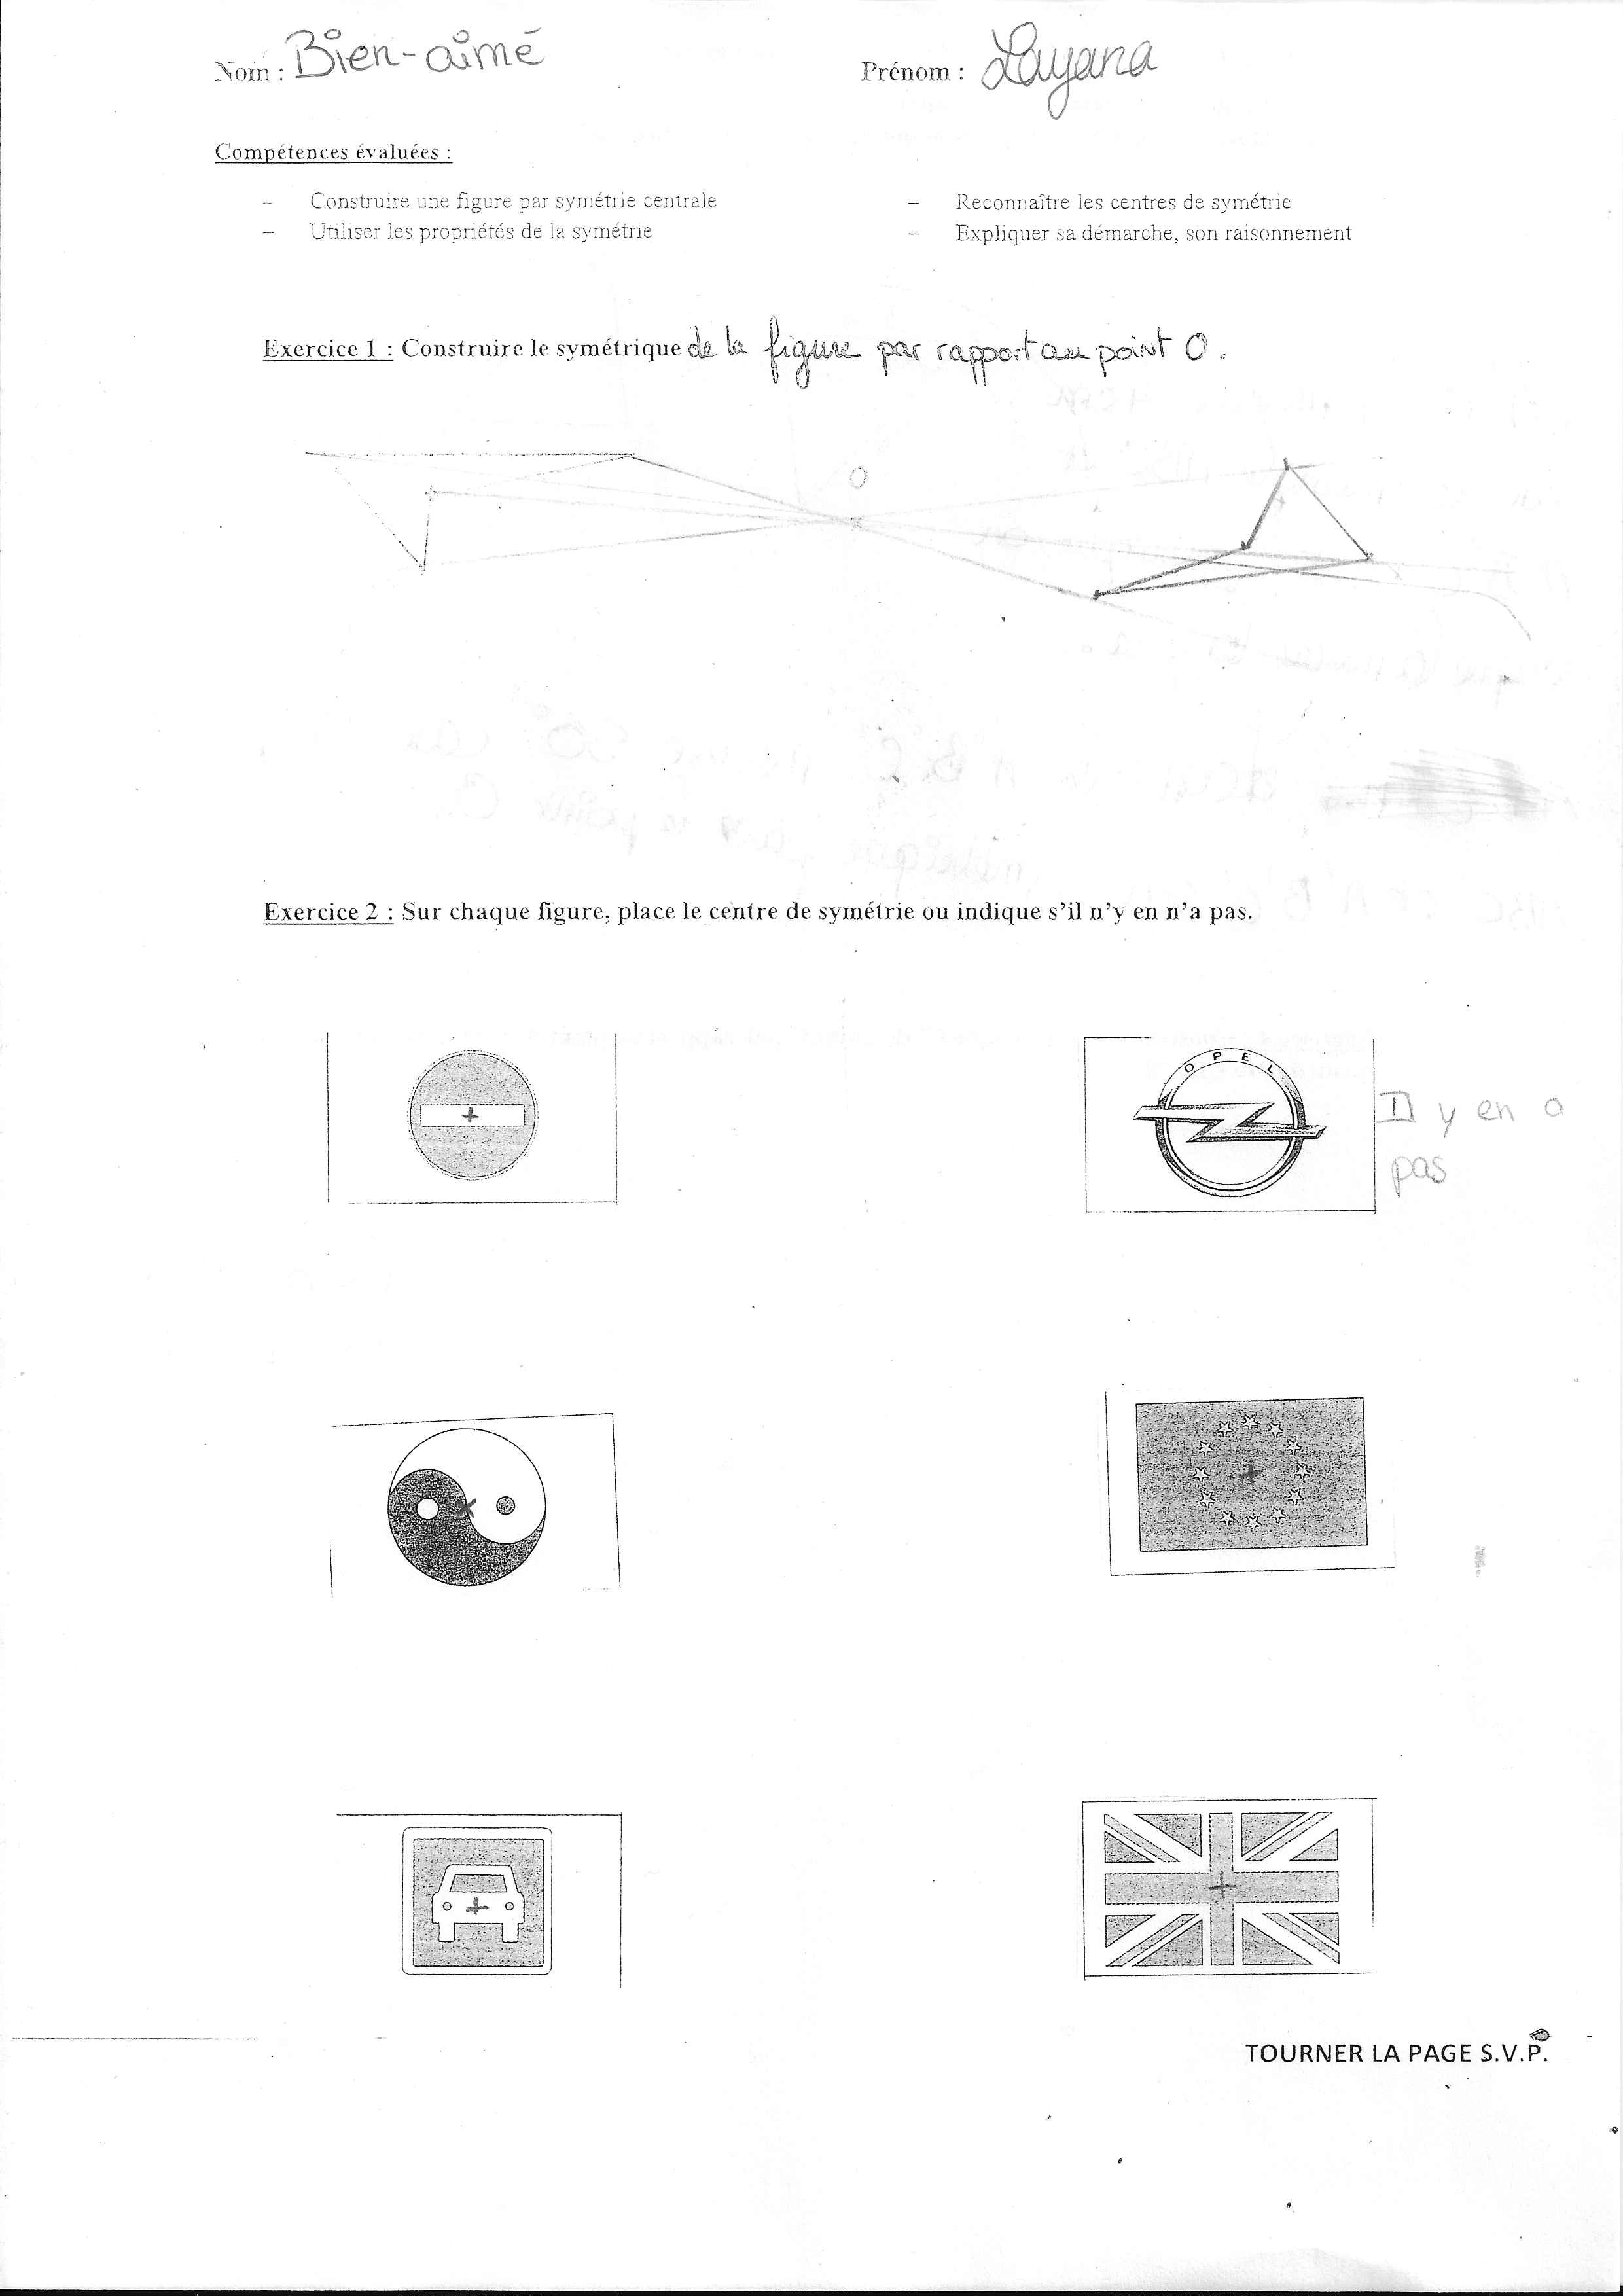
\includegraphics[scale=0.25]{img/Layana1.jpg}}}
%	\qquad
%	\subfloat{{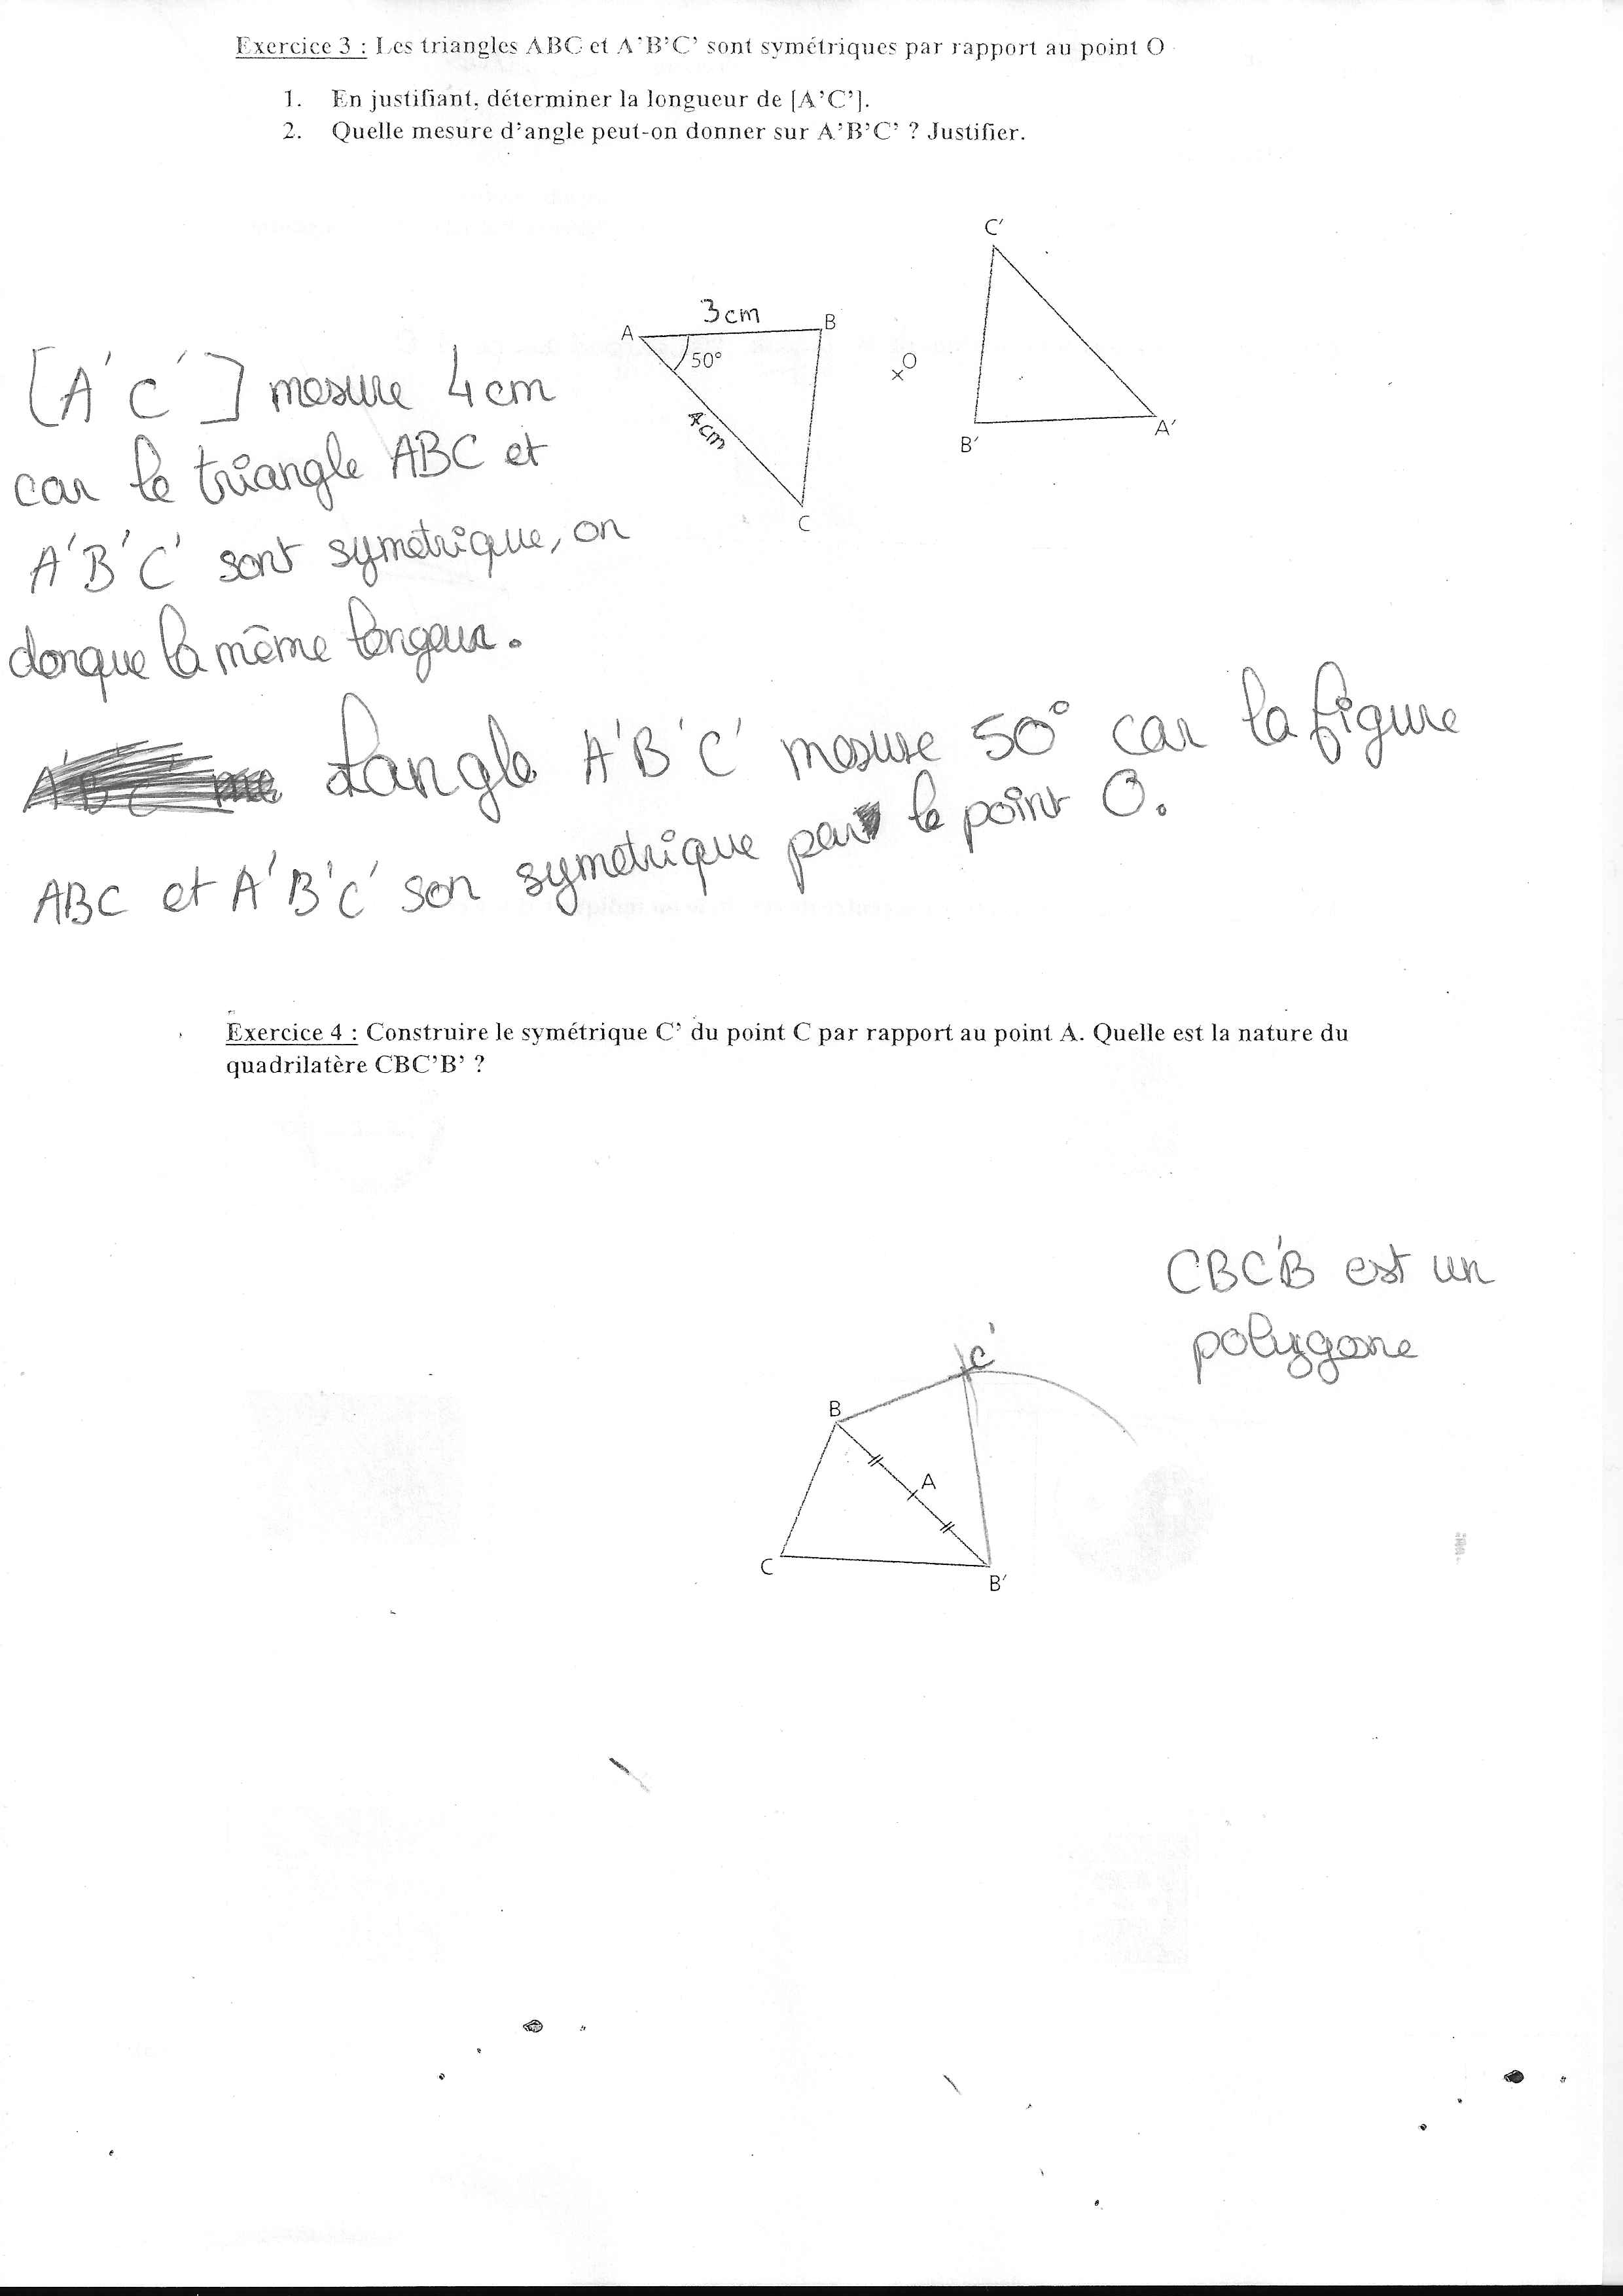
\includegraphics[scale=0.25]{img/Layana2.jpg}}}
%	\caption{Evaluation de Layana}
%	\label{fig:Eval_Layana}
%\end{figure}
\begin{figure}[!h]
	\center{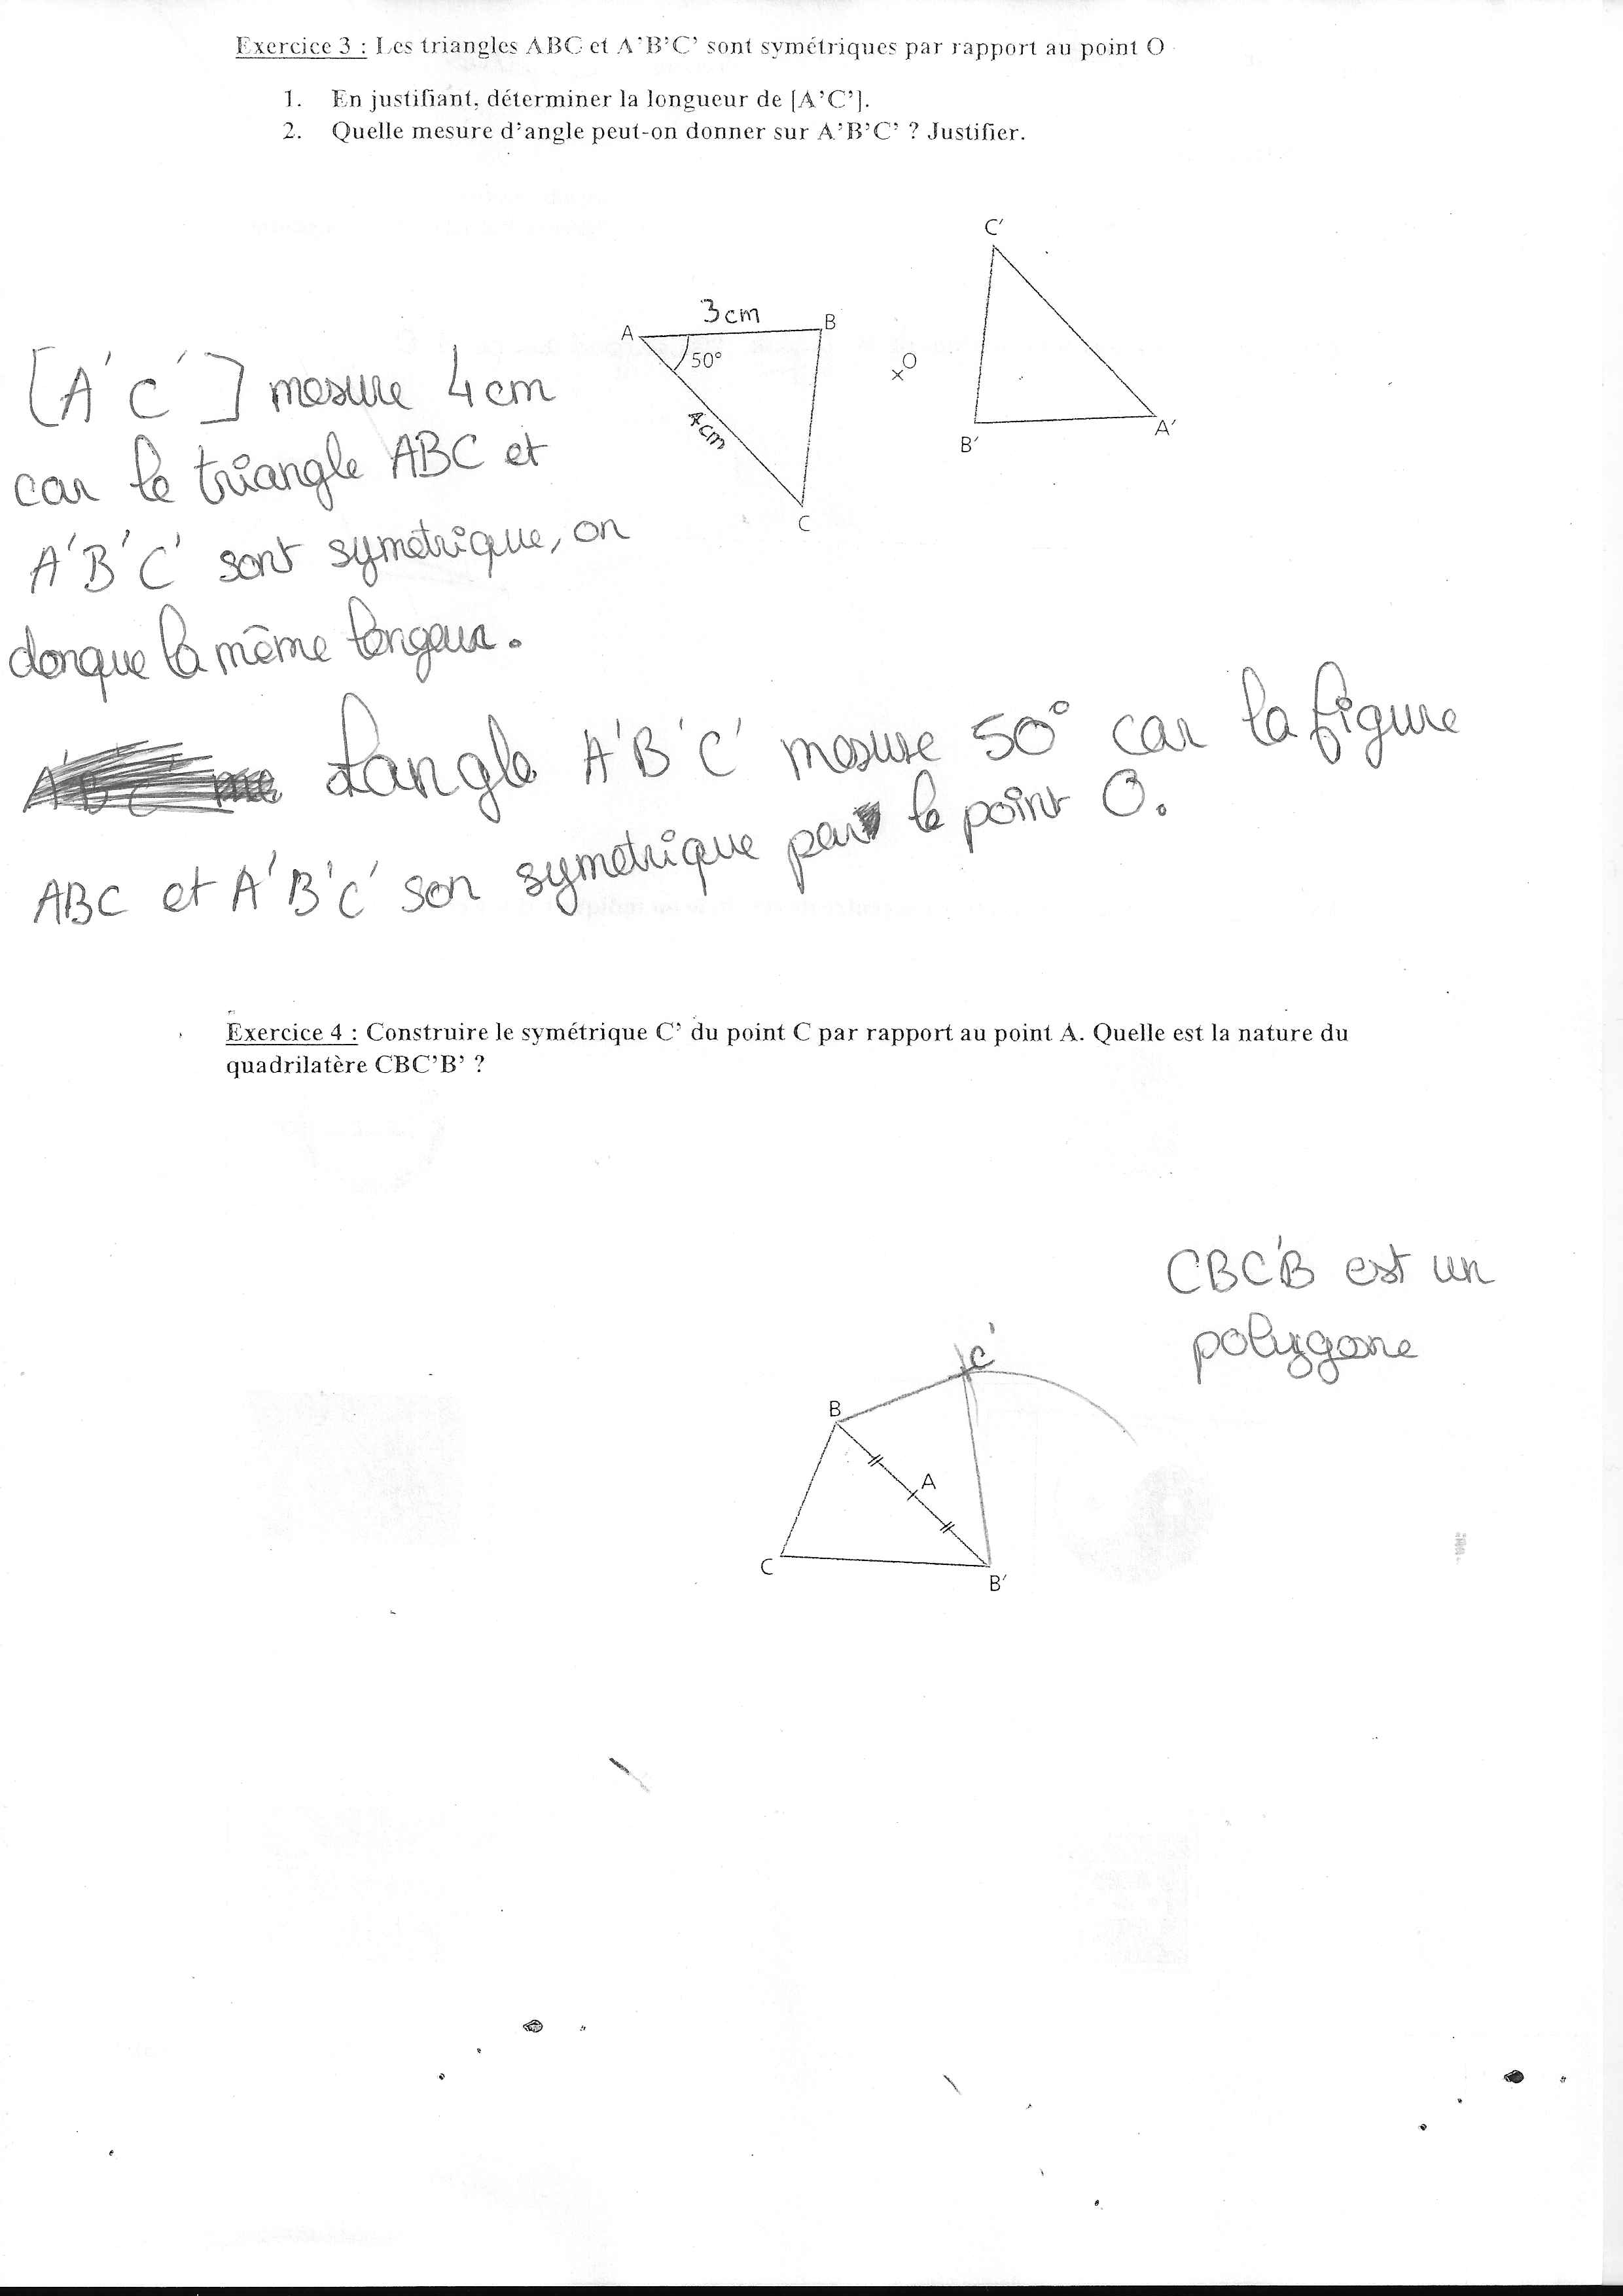
\includegraphics[scale=0.5]{img/Layana2.jpg}}
\end{figure}
\begin{figure}[!h]
	\center{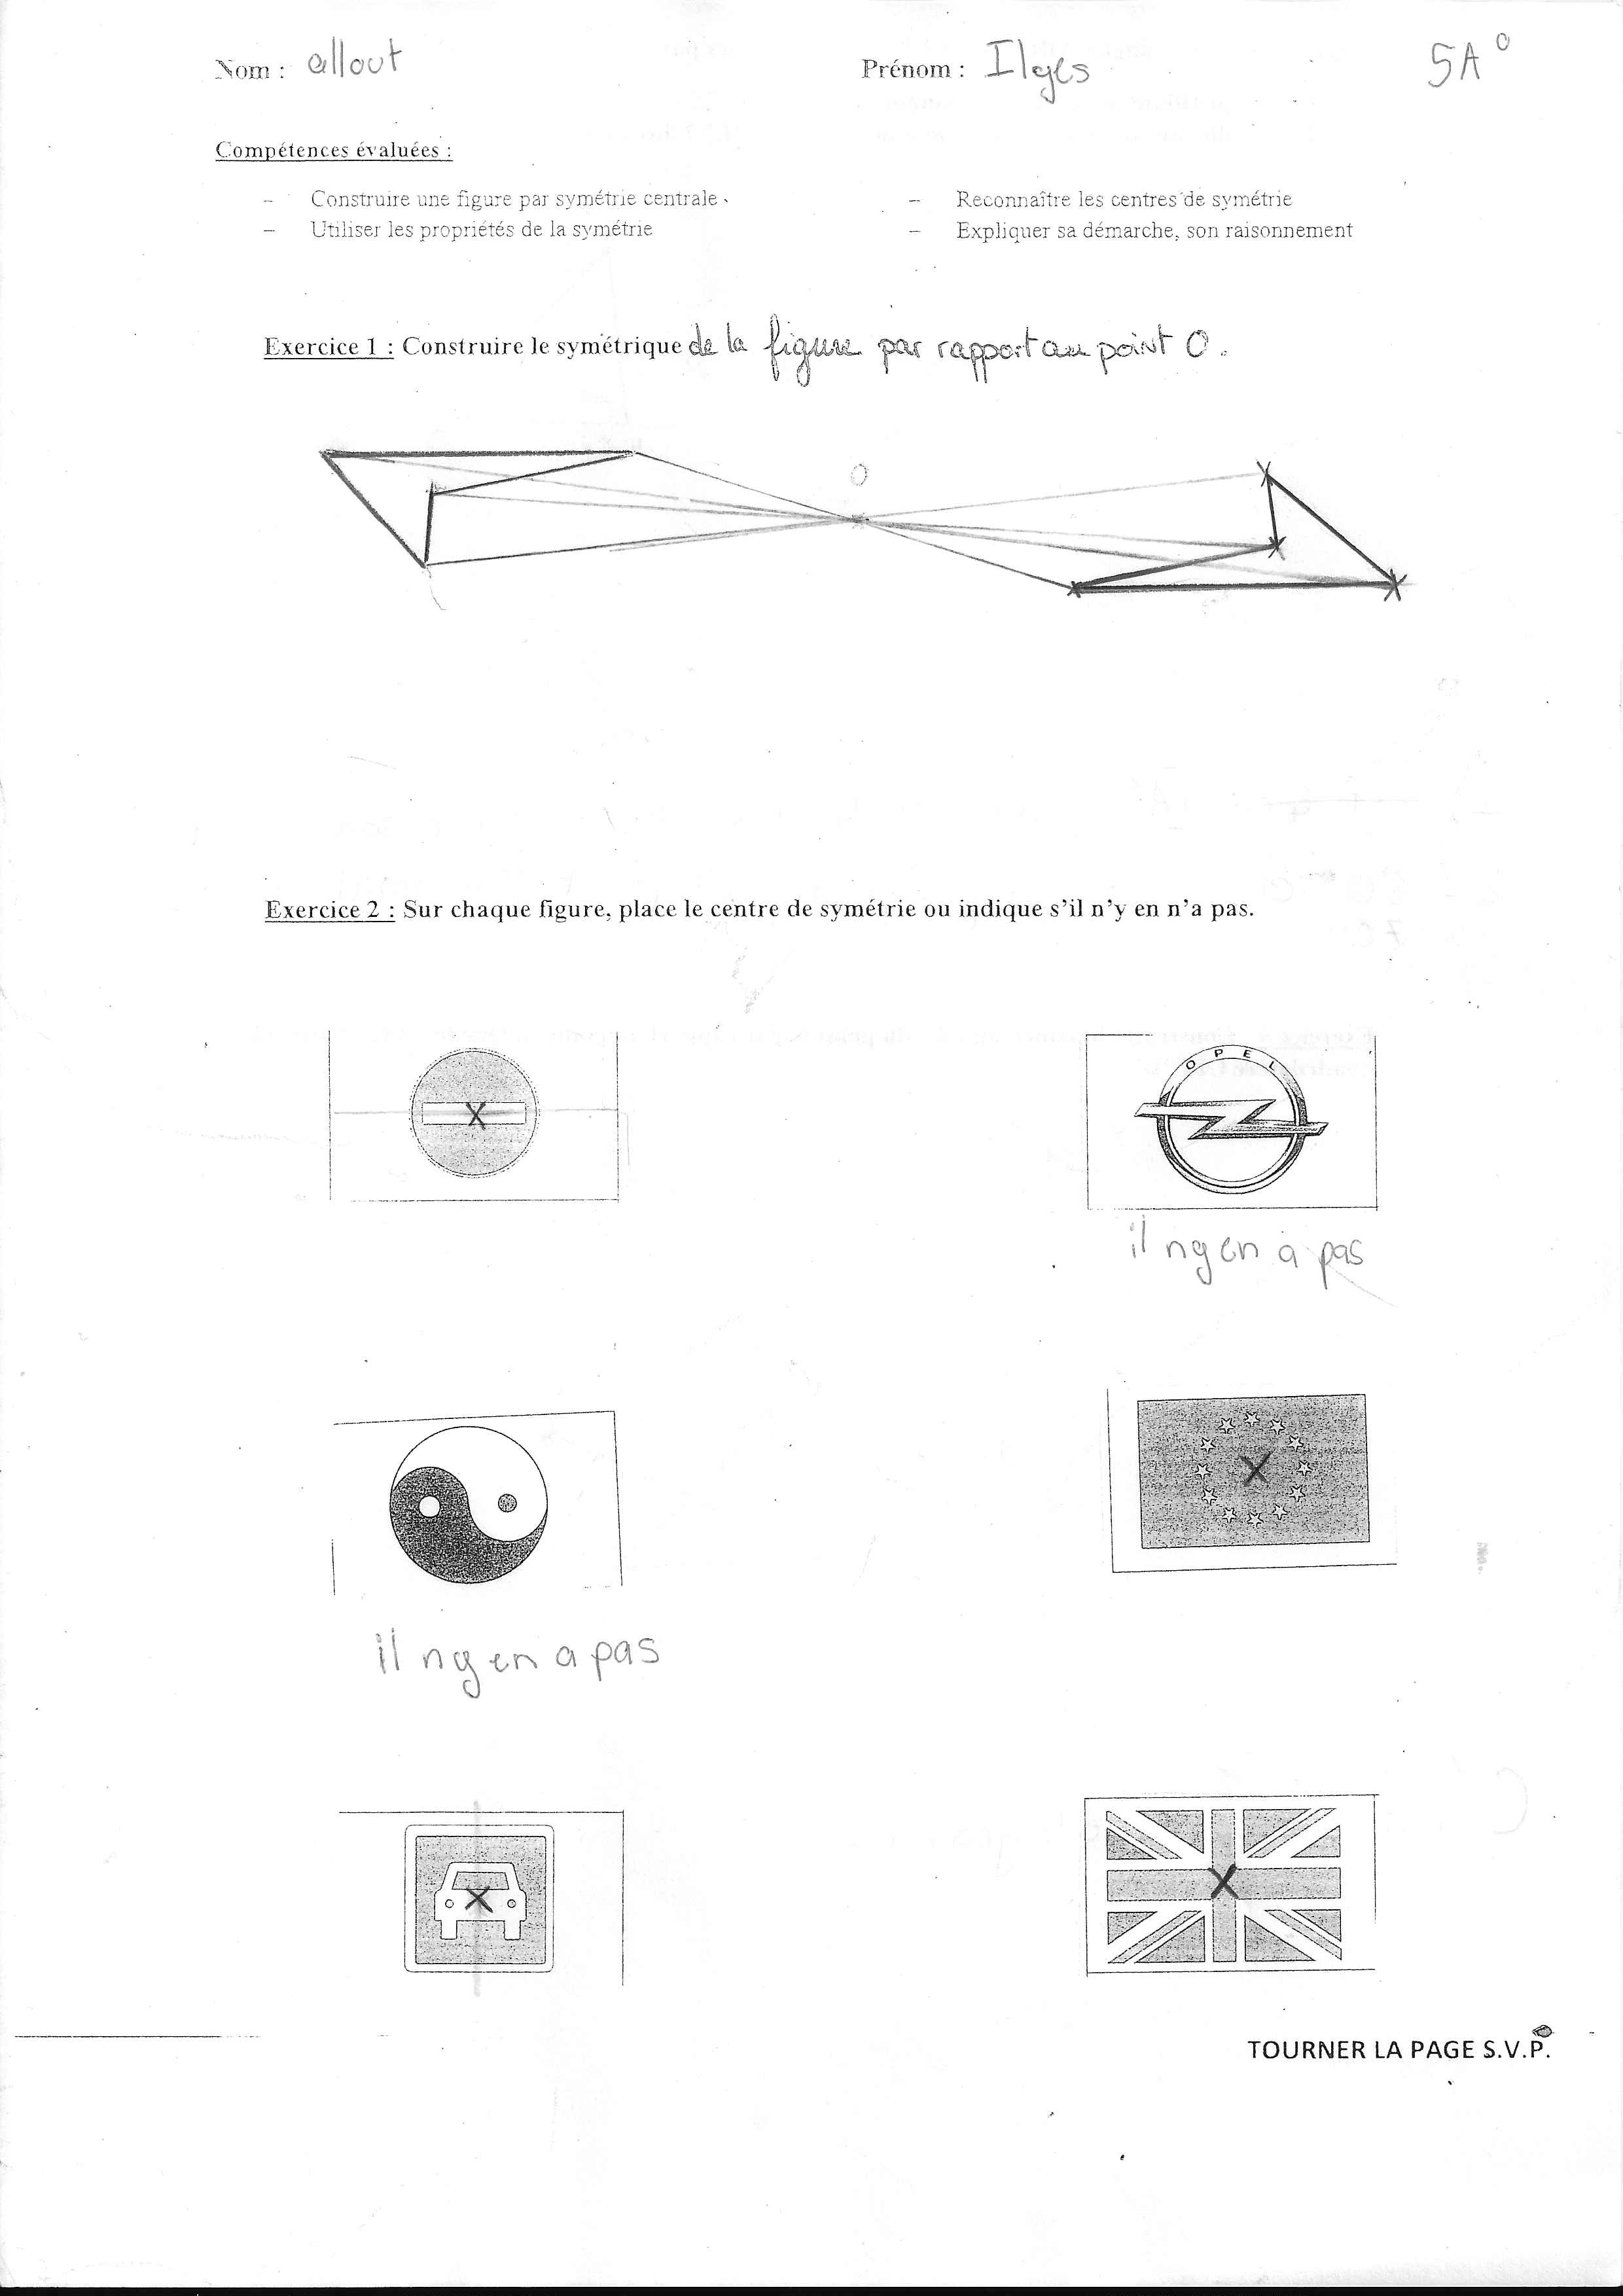
\includegraphics[scale=0.5]{img/Ilyes1.jpg}}
\end{figure}
\begin{figure}[!h]
	\center{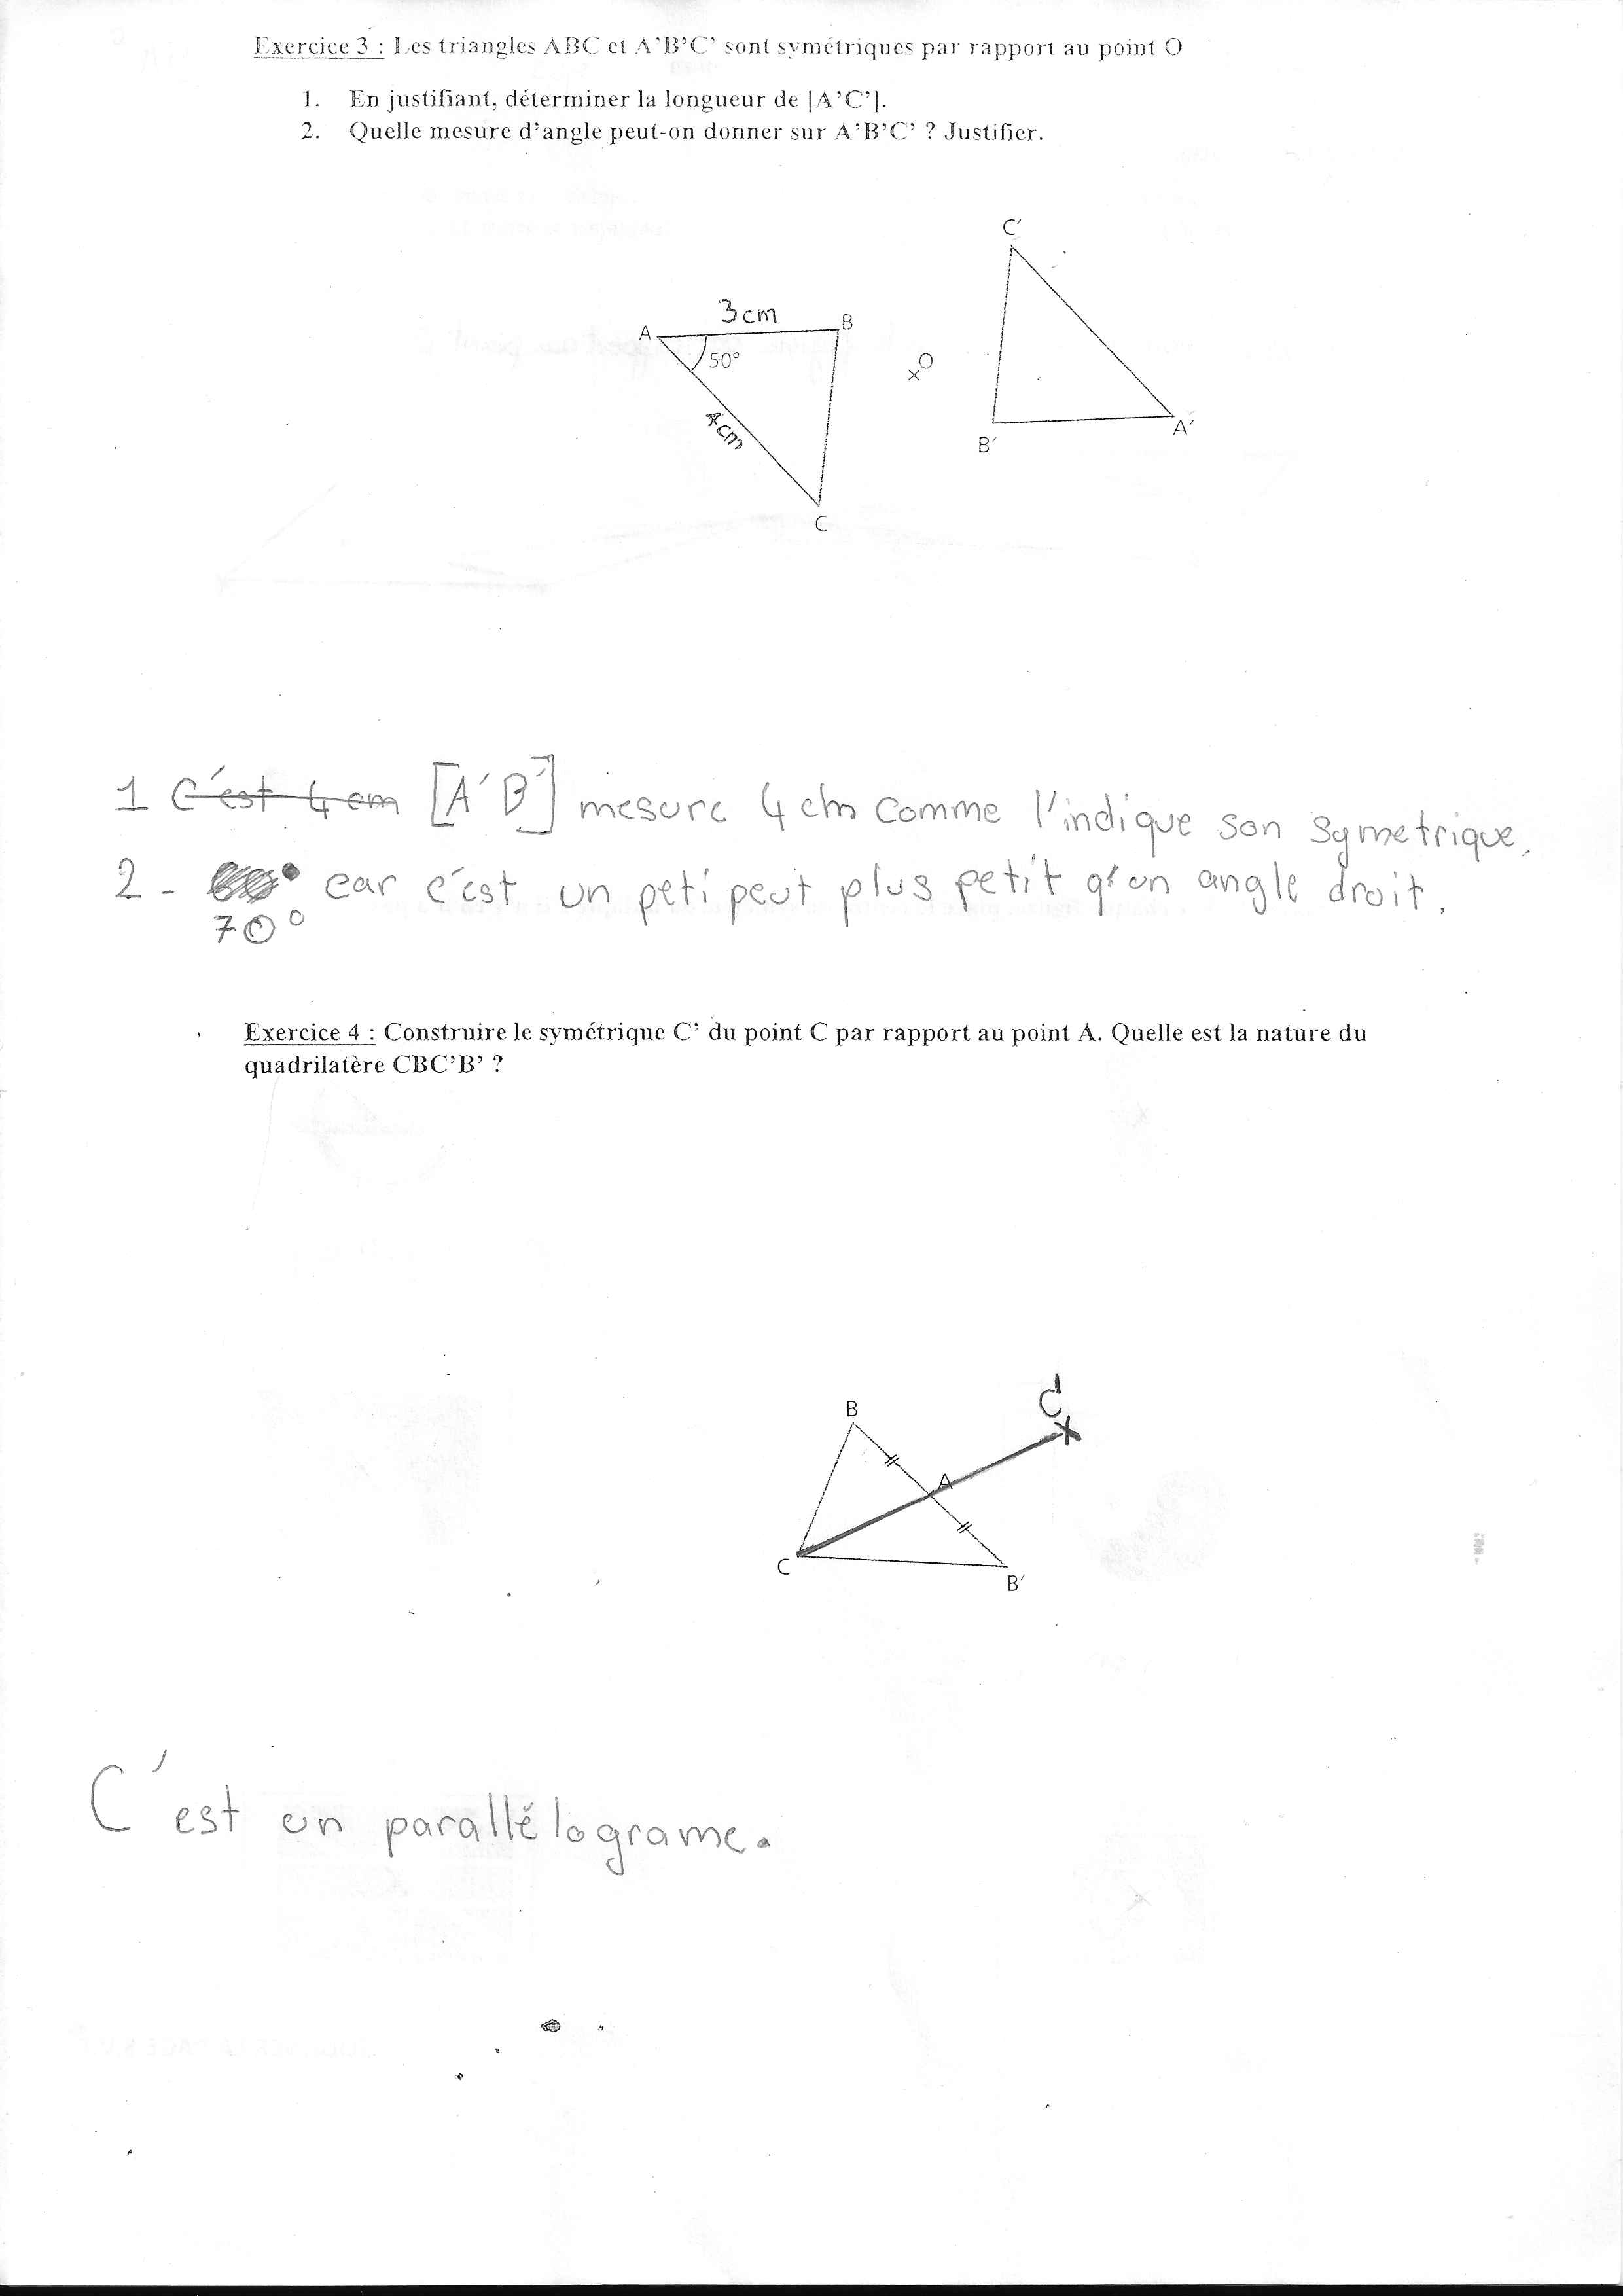
\includegraphics[scale=0.5]{img/Ilyes2.jpg}}
\end{figure}
\begin{figure}[!h]
	\center{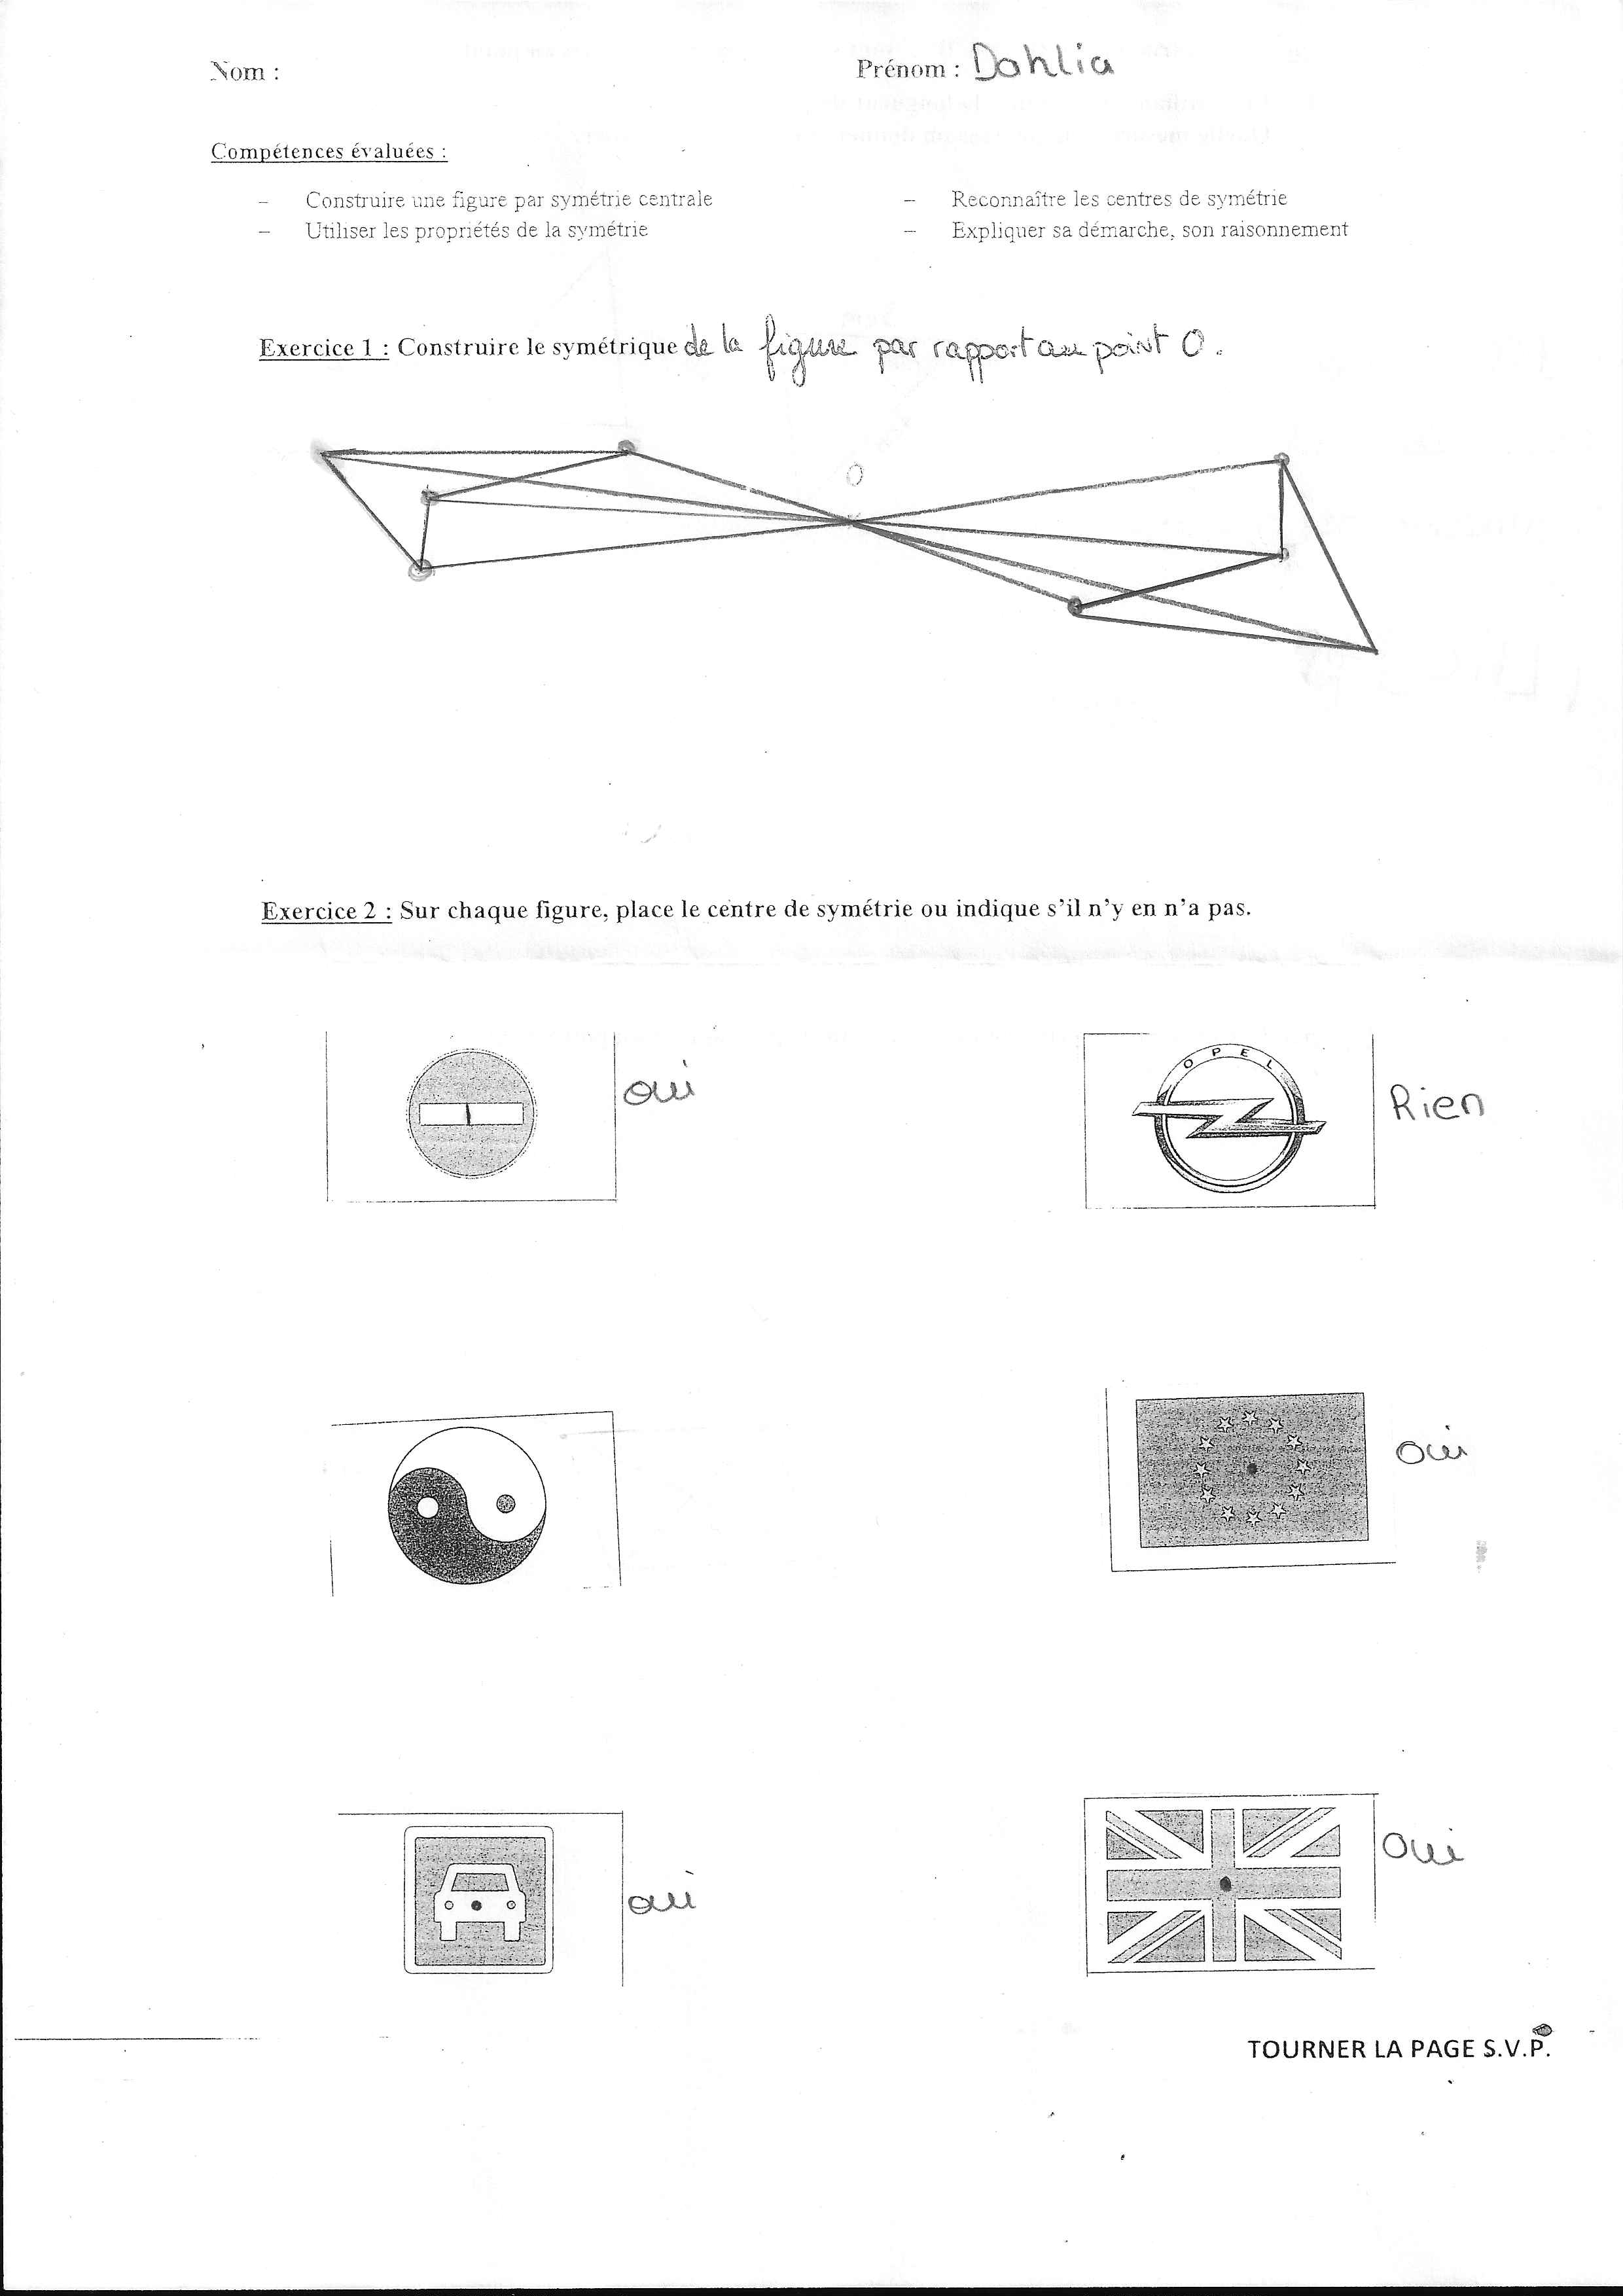
\includegraphics[scale=0.5]{img/dahlia1.jpg}}
\end{figure}
\begin{figure}[!h]
	\center{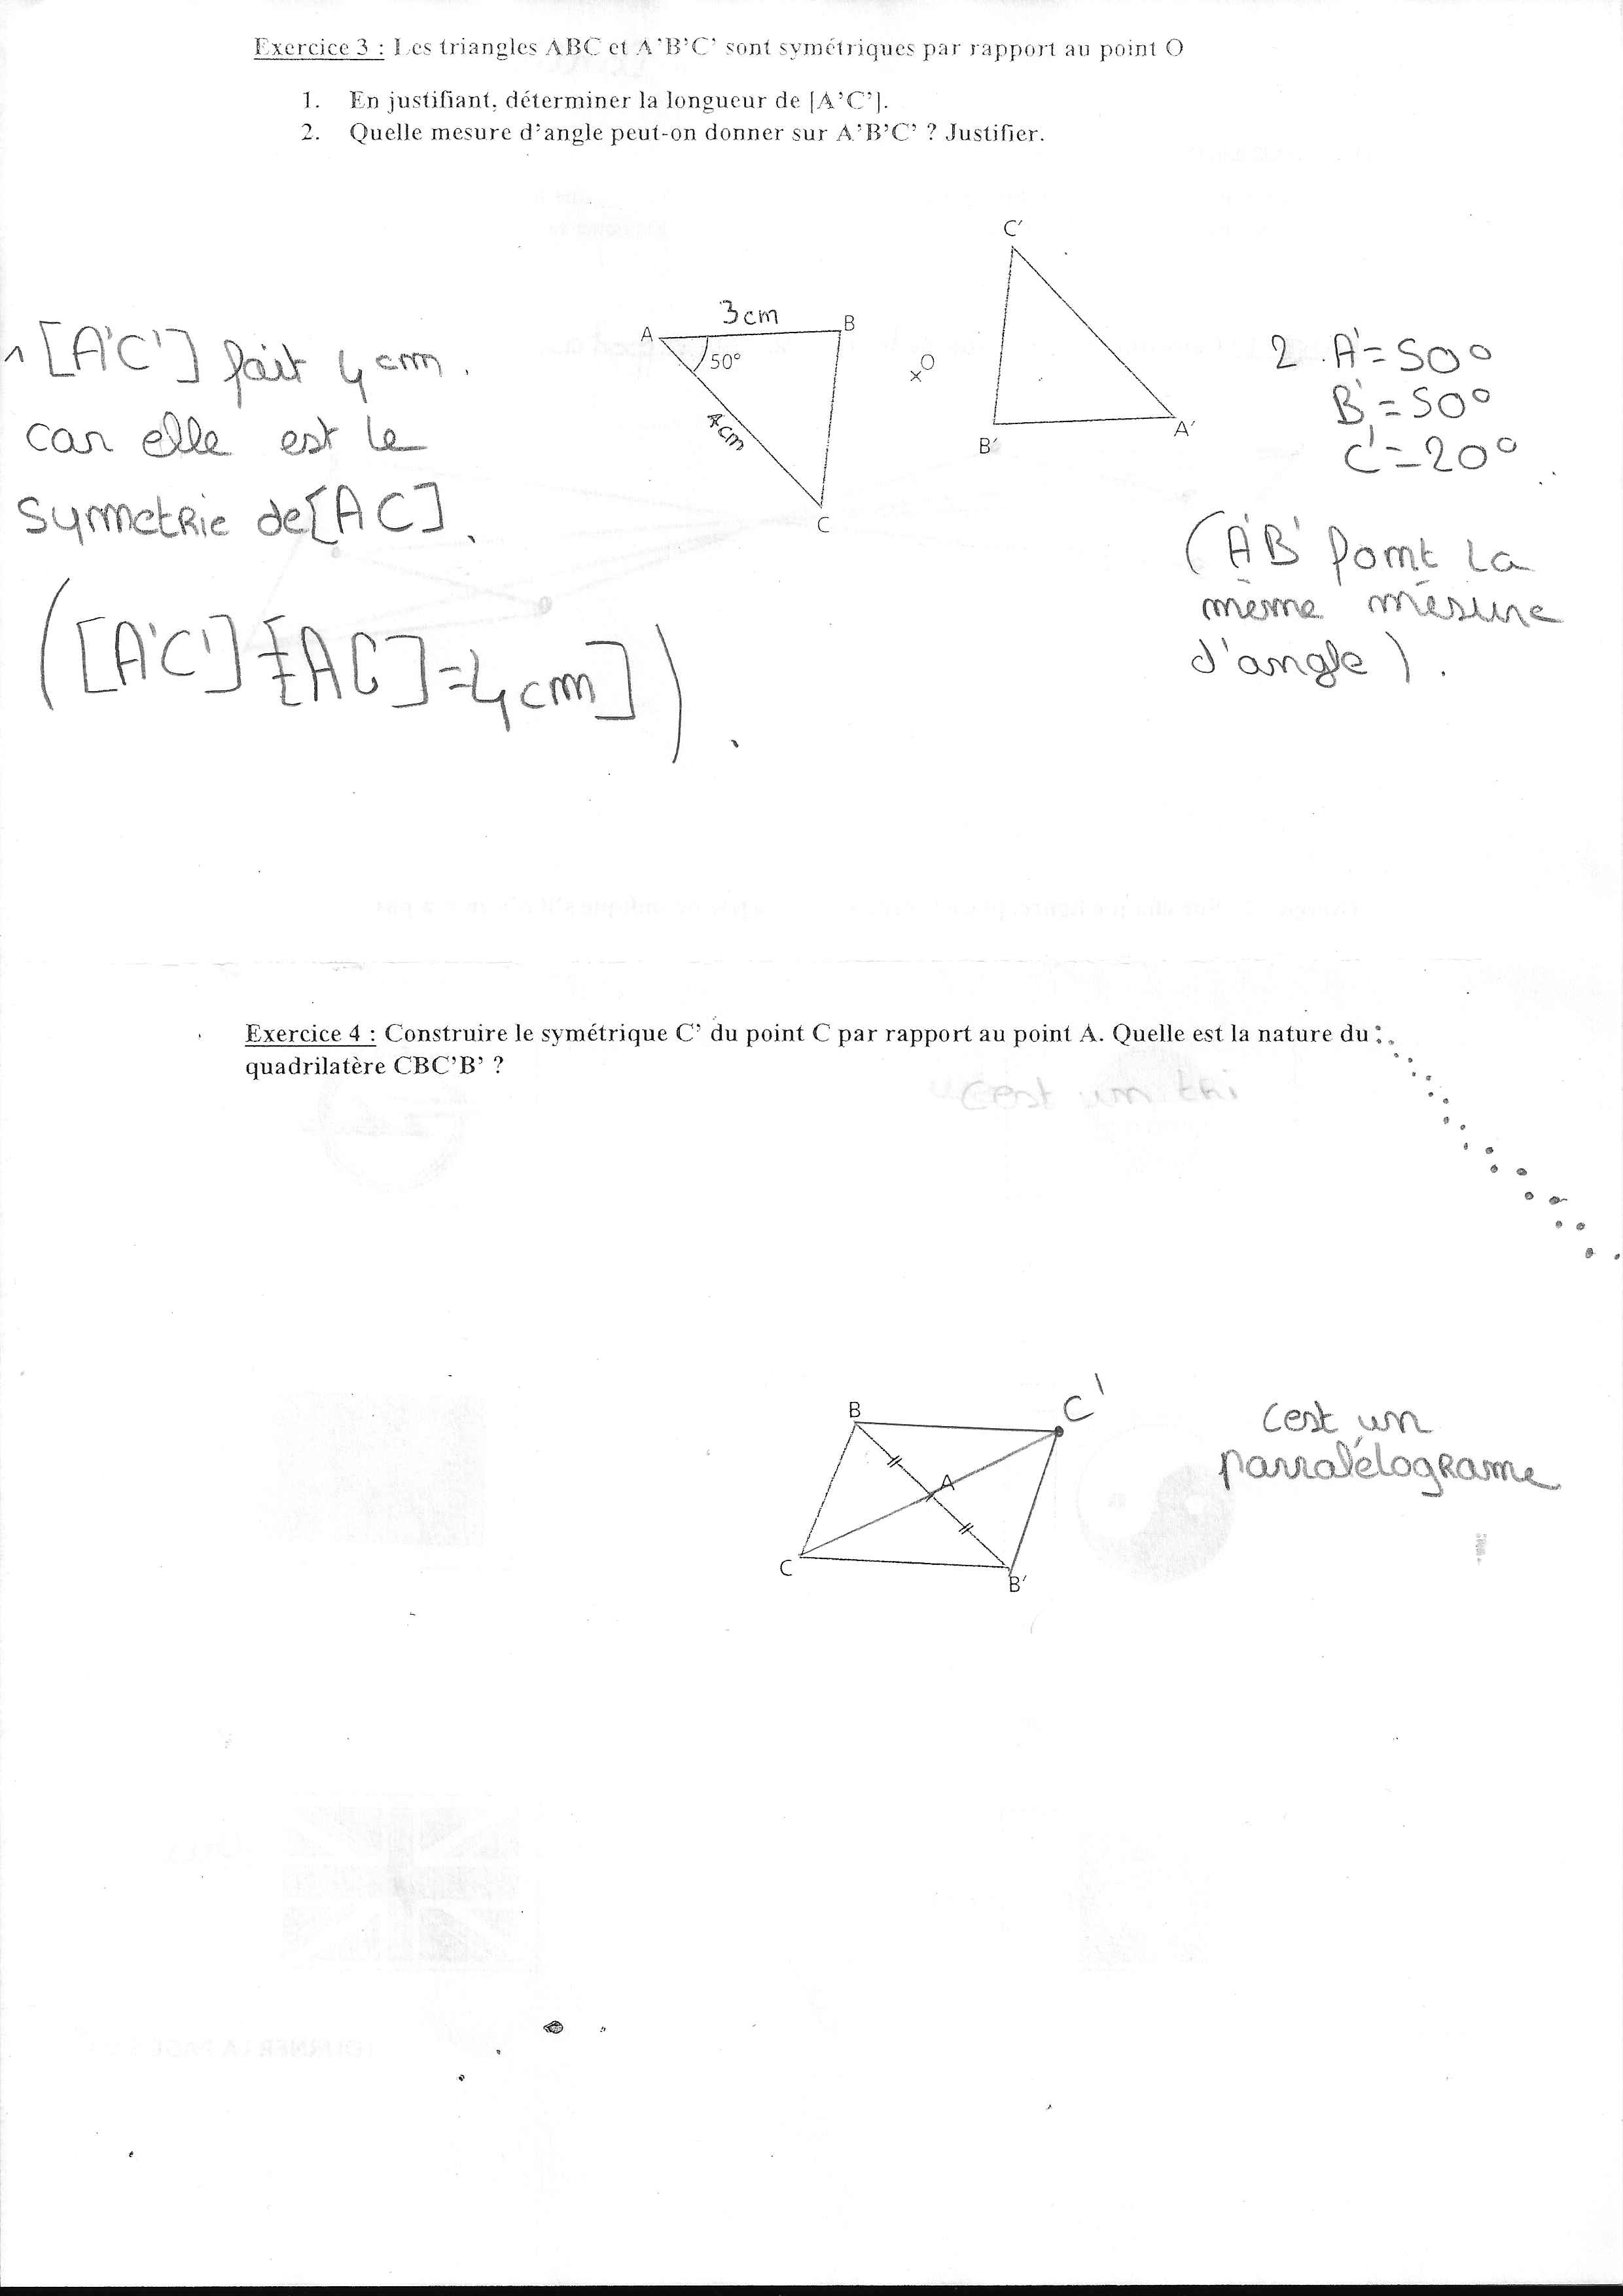
\includegraphics[scale=0.5]{img/dahlia2.jpg}}
\end{figure}
\subsubsection*{Evaluations}\label{Evaluations_ju}
\begin{figure}[!h]
	\center{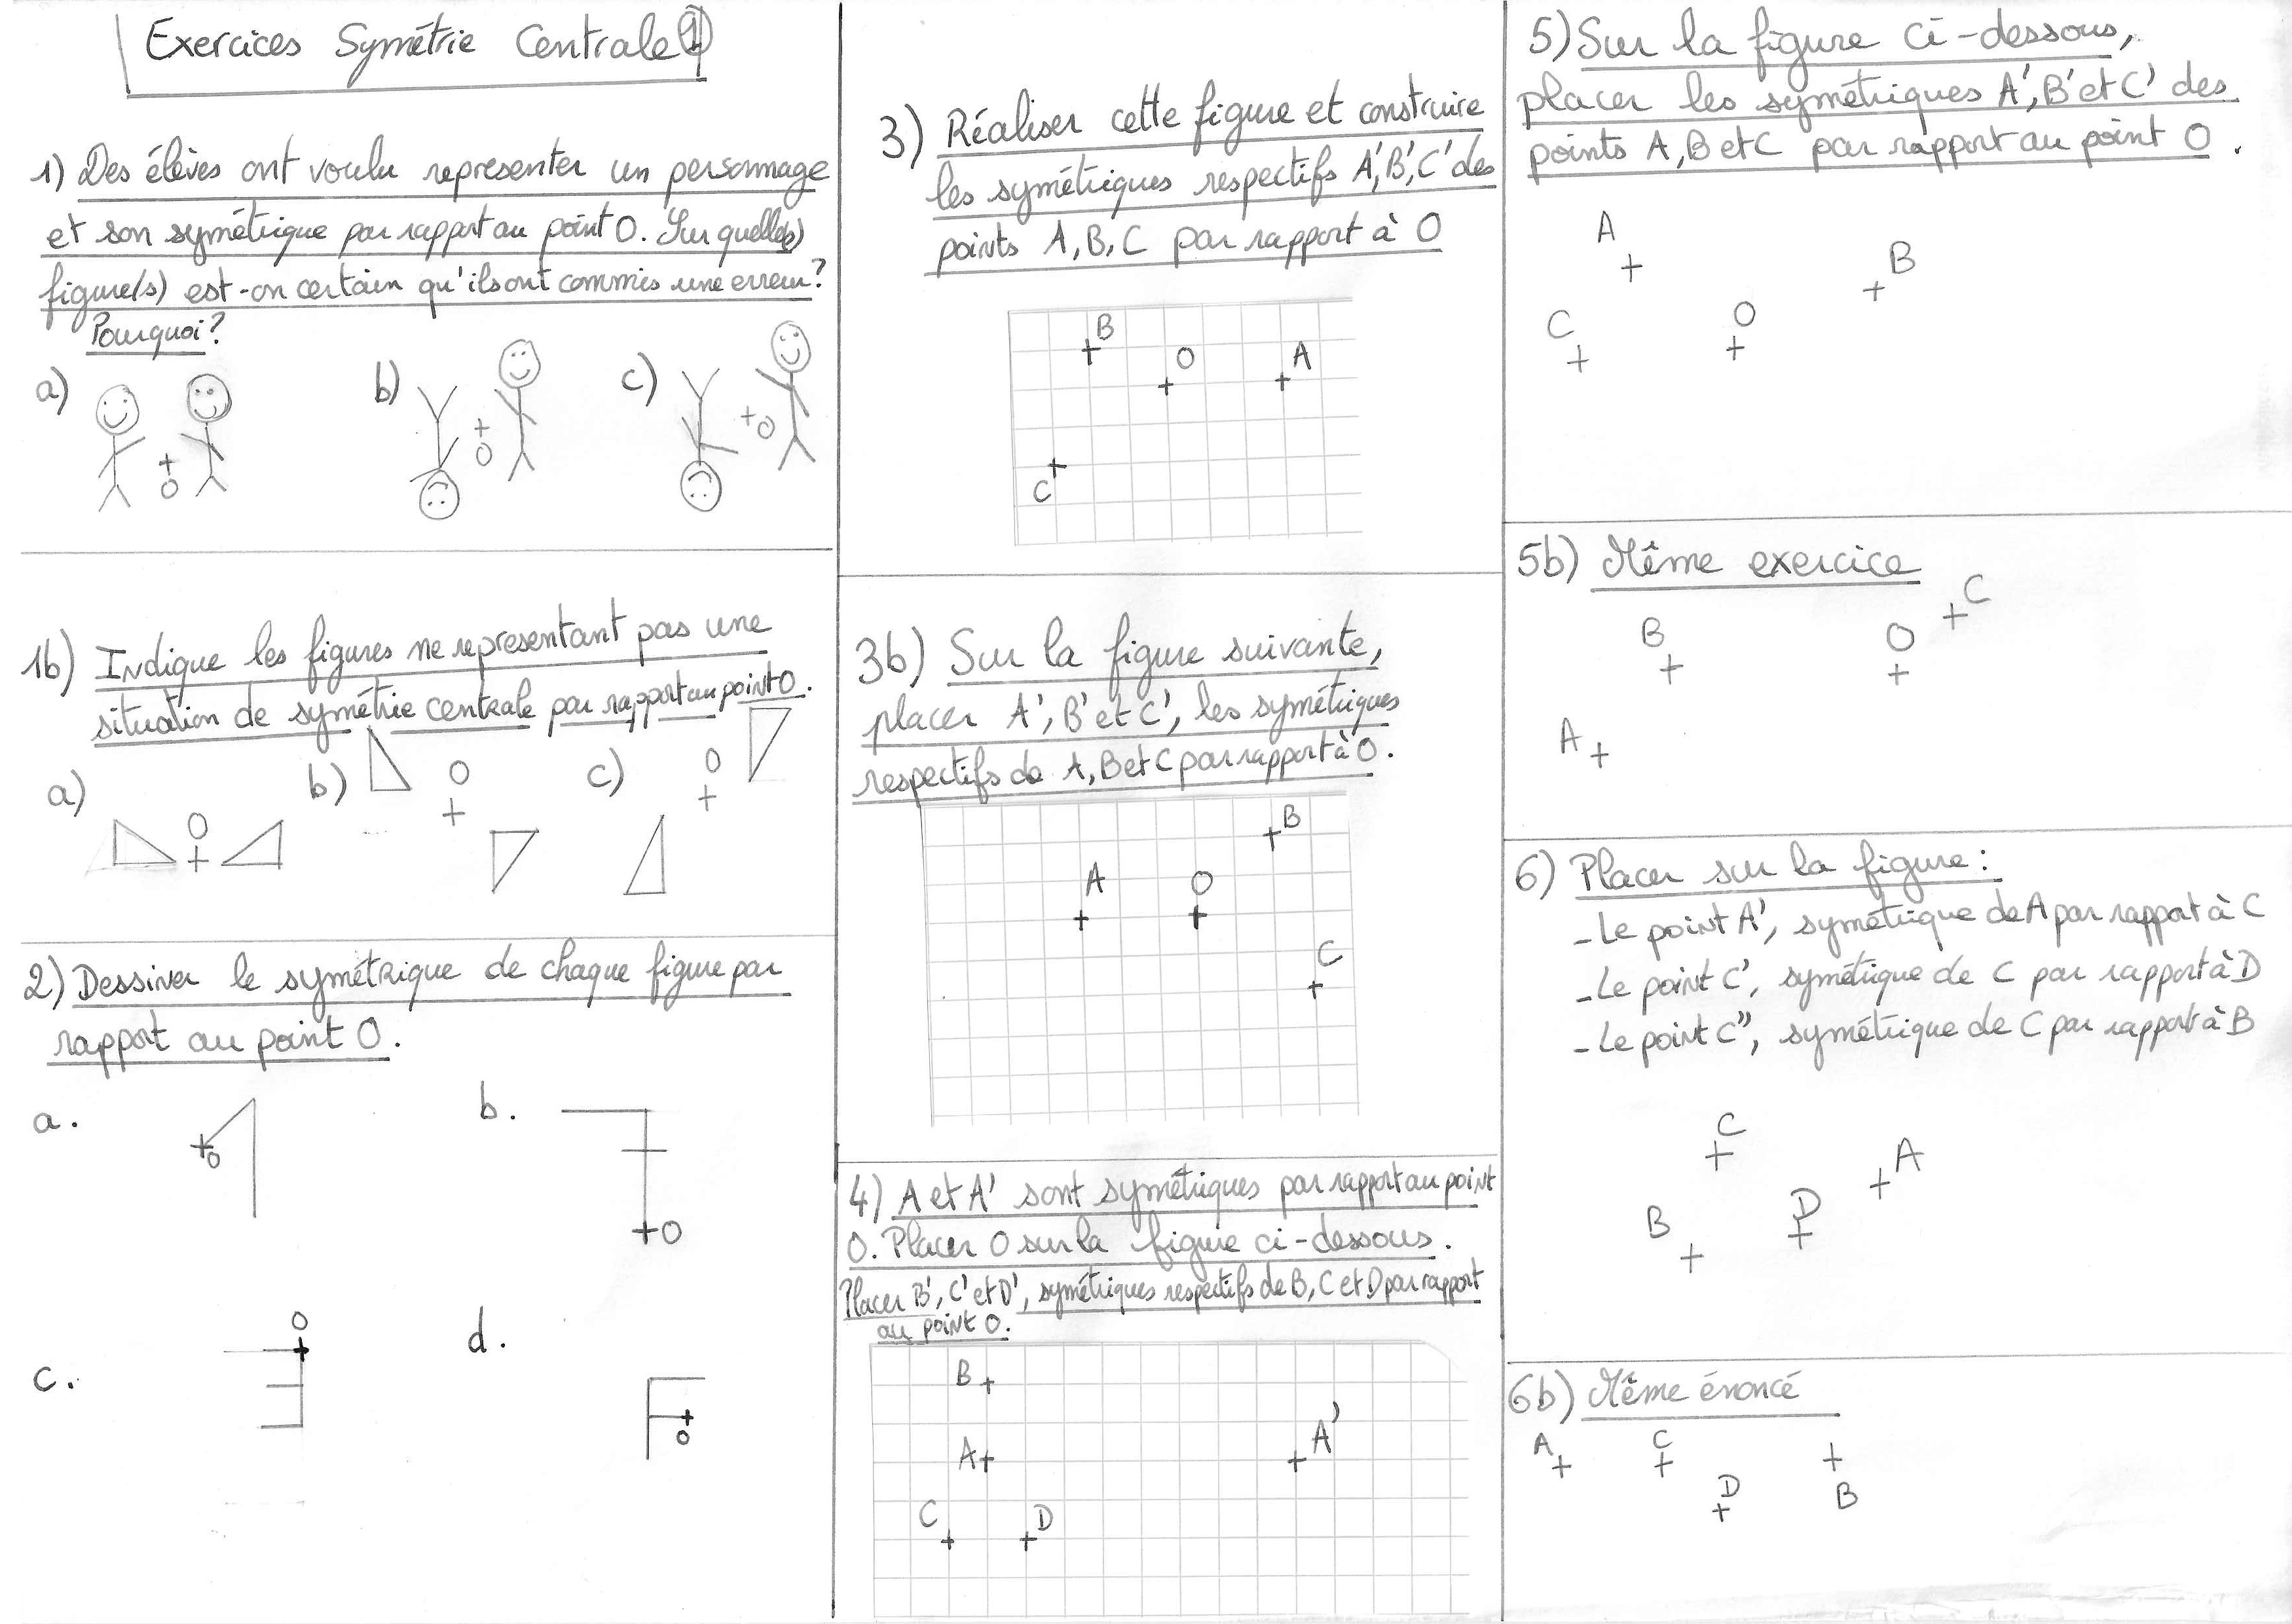
\includegraphics[scale=0.5]{img/Parcours_symetrie_julia1.jpg}}
\end{figure}